\section{Simulación de Lazo Abierto}
\section{Costo computacional de la simulación}

El objetivo de esta tesina es desarrollar un simulador capaz de ejecutarse en tiempo real, con el feedback del conductor dentro del lazo. Esta condición implica que el tiempo de cómputo necesario para avanzar la simulación un intervalo $\Delta t$ debe ser menor que $\Delta t$ medido en el reloj real. Esta sección apunta a medir en qué grado los modelos desarrollados cumplen con dicho requisito, y compara los integradores numéricos seleccionados en OpenModelica para este tipo de sistema. Primero se va a evaluar el sistema de lazo abierto, y luego se va a realizar una medición más específica con el entorno completo.


\subsection{Protocolo de medición}

Para obtener las mediciones se ejecutó cada uno de los tres modelos desarrollados (\verb|CivicEKCar|, \verb|E36Car| y \verb|Car|, este último referido como FF1600 por el monoplaza en el que se basa) realizando los mismos inputs, que generan una maniobra idéntica y deliberadamente exigente computacionalmente:

\begin{itemize}
    \item Horizonte de simulación de $10$ s.
    \item Comando de dirección al tope derecho ($\text{steer} = 1$) durante toda la maniobra.
    \item Acelerador al máximo ($\text{throttle} = 1$) desde el instante inicial.
    \item Aplicación del freno al máximo ($\text{brake} = 1$) a partir de $t = 5$ s.
\end{itemize}

La maniobra combina saturación simultánea de demanda longitudinal y lateral ya que el vehículo acelera en un giro de radio mínimo (en teoría) hasta la mitad del intervalo y frena en esa misma condición durante el resto. Es un caso desfavorable de forma intencional, ya que lleva al neumático al límite del círculo de fricción, donde la saturación de la fuerza de contacto introduce la no linealidad más severa del modelo.

Cada modelo se evaluó sobre dos geometrías de terreno, una superficie plana y otra que generaba una superficie sinusoidal, con los dos integradores mencionados anteriormente (DASSL y CVODE), con el agregado de \verb|gbode| en algunos casos, con el objetivo de comparar contra otra familia de solver. Se registran dos magnitudes: el tiempo \textit{total}, que incluye la inicialización del sistema y la escritura de resultados, y el tiempo de \textit{simulación}, correspondiente al tiempo de avance de la integración.  Las mediciones se realizaron sobre el ejecutable ya compilado, de modo que el tiempo de traducción y compilación del modelo queda excluido, ya que no son relevantes a la ejecución en tiempo real.

\subsection*{Resultados}

La tabla~\ref{tab:tiempos} grafica las mediciones. El símbolo $\dagger$ marca las ejecuciones que abortaron antes de alcanzar los $10$ s de simulación establecidos, en esos casos el valor registrado corresponde al tiempo total de ejecución de la simulación hasta la falla y por lo tanto no es una medida de tiempo comparable con las ejecuciones que completaron correctamente.


\begin{table}[H]
\centering
\begin{tabular}{llcccccc}
\hline
 & & \multicolumn{3}{c}{Tiempo total (s)} & \multicolumn{3}{c}{Tiempo de simulación (s)} \\
Terreno & Solver & Civic & E36 & FF1600 & Civic & E36 & FF1600 \\
\hline
\multirow{2}{*}{Plano}
 & DASSL & 1{,}468 & 1{,}658 & 0{,}396$^\dagger$ & 1{,}152 & 1{,}339 & 0{,}329$^\dagger$ \\
 & CVODE & 0{,}793 & 0{,}654 & 0{,}780 & 0{,}756 & 0{,}619 & 0{,}741 \\
\hline
\multirow{2}{*}{Sinusoidal}
 & DASSL & 0{,}323$^\dagger$ & 0{,}502$^\dagger$ & 2{,}353$^\dagger$ & 0{,}238$^\dagger$ & 0{,}411$^\dagger$ & 1{,}984$^\dagger$ \\
 & CVODE & 4{,}184 & 1{,}867 & 1{,}486 & 4{,}095 & 1{,}805 & 1{,}435 \\
\hline
\end{tabular}

\caption[Tiempos de ejecución de los modelos de vehículo]{Tiempos de ejecución para una maniobra de $10$ s con dirección al tope, acelerador máximo y frenada máxima a partir de $t = 5$ s, con tolerancia relativa $10^{-6}$. $^\dagger$ La ejecución abortó antes de completar la simulación, el valor indica el tiempo hasta la falla y no es comparable con el de una corrida completa.}
\label{tab:tiempos}
\end{table}

La figura~\ref{fig:tiempos} representa gráficamente los tiempos de simulación de la tabla. Se omiten las barras de las ejecuciones que no completaron correctamente.

\begin{figure}[H]
\centering
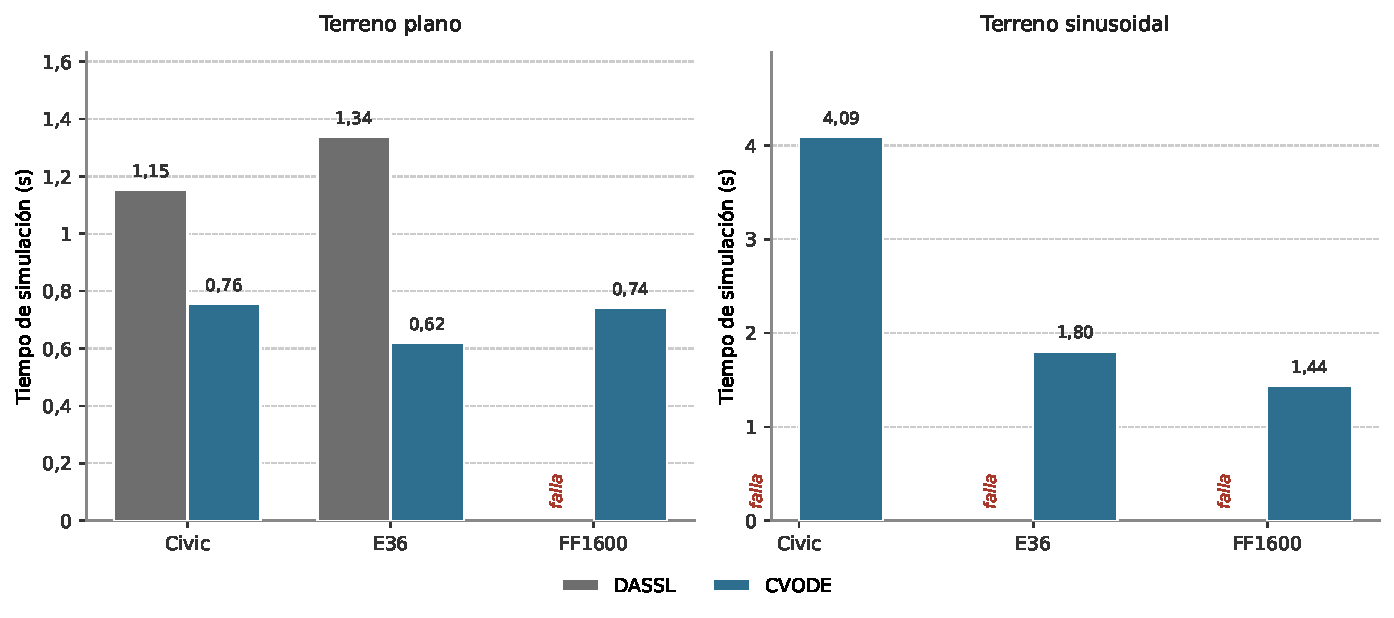
\includegraphics[width=\textwidth]{img/tiempos_simulacion.pdf}


\caption[Tiempo de simulación por vehículo, solver y terreno]{Tiempo de simulación para la maniobra de $10$ s. Las entradas marcadas como \textit{falla} corresponden a ejecuciones que abortaron antes de completar la simulación y por lo tanto no se grafican: DASSL falla con el modelo FF1600 sobre terreno plano y con los tres vehículos sobre terreno sinusoidal. CVODE completa las seis configuraciones.}
\label{fig:tiempos}
\end{figure}

El resultado más interesante para la tesina no es el tiempo absoluto, si no, como se compara este con el tiempo total de la simulación, ya que una relación menor a 1x limita la capacidad de ejecutar un entorno en tiempo real. La Figura~\ref{fig:tiemporeal} expresa las mediciones de CVODE (ya que fue el único integrador en completar todas las configuraciones) como factor un coeficiente entre el tiempo total de la simulación y el tiempo que tardó en ejecutarse. La línea discontinua en $1\times$ marca la frontera del tiempo real: por encima de ella la simulación avanza más rápido que el reloj y, por lo tanto, admite operación con el conductor dentro del lazo.


\begin{figure}[H]
\centering
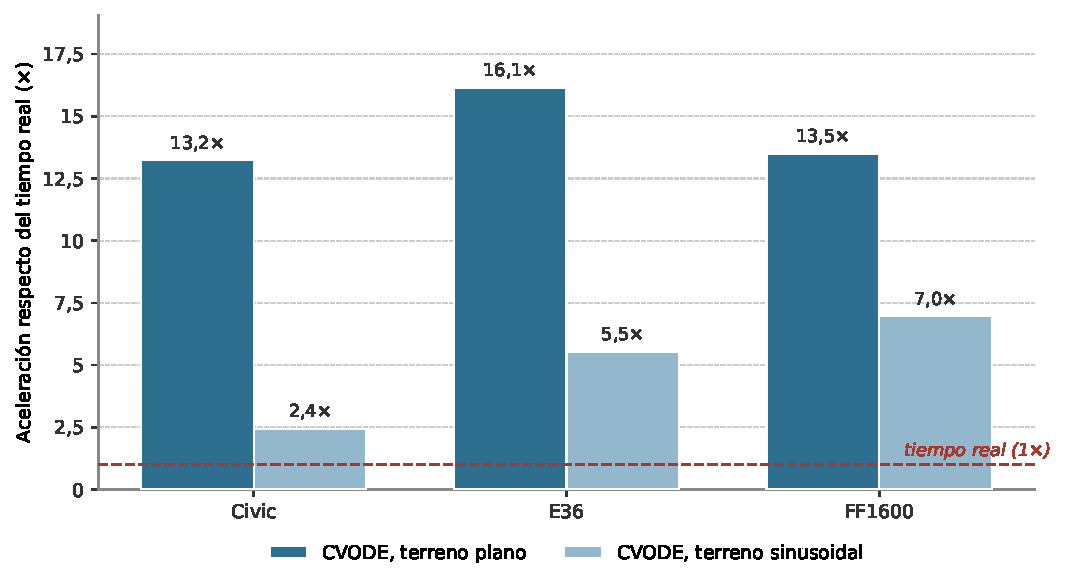
\includegraphics[width=0.86\textwidth]{img/tiempo_real.pdf}
\caption[Aceleración respecto del tiempo real]{Factor de aceleración respecto del tiempo real de los tres modelos de vehículo con CVODE, definido como el cociente entre el horizonte simulado ($10$ s) y el tiempo de cómputo. La línea discontinua marca el umbral de tiempo real: todos los casos se sitúan por encima, con márgenes entre $2{,}4\times$ y $16{,}1\times$.}
\label{fig:tiemporeal}
\end{figure}

\subsection{Complejidad de los modelos}

Para interpretar mejor los tiempos, conviene tener una medida del tamaño de cada modelo. La tabla~\ref{tab:complejidad} muestra el número de ecuaciones del sistema plano (obtenido usando la instrucción \verb|checkModel| de OpenModelica) junto con el número de estados continuos e indicadores de evento (leídos de la descripción \verb|modelDescription.xml| del FMU exportado).

\begin{table}[H]
\centering
\begin{tabular}{lrrrr}
\hline
Modelo & Ecuaciones & Triviales & Estados & Ind. de evento \\
\hline
\verb|Car| (FF1600) & 12\,269 & 8\,585 & 30 & 8 \\
\verb|CivicEKCar|   & 12\,269 & 8\,584 & 30 & 8 \\
\verb|E36Car|       &  9\,897 & 6\,746 & 30 & 8 \\
\hline
\end{tabular}

\caption[Complejidad de los modelos de vehículo]{Tamaño de cada modelo de vehículo. Las ecuaciones triviales son las que el compilador resuelve por sustitución directa y no llegan al sistema que resuelve el integrador. Los estados continuos y los indicadores de evento se obtuvieron de la descripción del FMU exportado de cada modelo.}
\label{tab:complejidad}
\end{table}

El dato más relevante de la tabla es que los tres vehículo tienen exactamente el mismo número de estados continuos, a pesar de que utilizan topologías distintas. Esto es debido al uso del componente  \verb|JointRRR| señalada en la Sección~\ref{sec:method}: al resolver analíticamente el bucle cinemático, no introduce restricciones ni variables de estado adicionales. Los treinta estados corresponden a los seis grados de libertad del chasis, los cuatro recorridos de suspensión y los cuatro giros de rueda, con sus respectivas derivadas, independientemente de que la suspensión sea de doble triángulo, McPherson o multibrazo. A notar también de que tanto el FF1600 como el CivicEKCar contienen la misma cantidad de ecuaciones, a pesar de ser vehículos completamente distintos en papel, sin embargo, su topología de suspensión es la misma (doble triángulo en las cuatro esquinas). 


\subsection{Sensibilidad a la tolerancia}

La tolerancia relativa del integrador es el parámetro que controla el compromiso entre exactitud y costo computacional. Para tener una mejor idea sobre que valor utilizar, se repitió la maniobra sobre el terreno sinusoidal (ya que es el más exigente) con CVODE y tolerancias de $10^{-4}$, $10^{-6}$ y $10^{-8}$. Los resultados se presentan en la Tabla~\ref{tab:tolerancia} y la Figura~\ref{fig:tolerancia}.

\begin{table}[H]
\centering
\begin{tabular}{lcccccc}
\hline
 & \multicolumn{3}{c}{Tiempo total (s)} & \multicolumn{3}{c}{Tiempo de simulación (s)} \\
Tolerancia & Civic & E36 & FF1600 & Civic & E36 & FF1600 \\
\hline
$10^{-4}$ & 2{,}473 & 1{,}015 & 0{,}963 & 2{,}232 & 0{,}804 & 0{,}728 \\
$10^{-6}$ & 4{,}767 & 1{,}555 & 1{,}487 & 4{,}549 & 1{,}375 & 1{,}271 \\
$10^{-8}$ & 7{,}721 & 2{,}582 & 2{,}446 & 7{,}508 & 2{,}405 & 2{,}232 \\
\hline
\end{tabular}
\caption[Sensibilidad del costo a la tolerancia del integrador]{Tiempos con CVODE sobre terreno sinusoidal para tres tolerancias relativas.}
\label{tab:tolerancia}
\end{table}

\begin{figure}[H]
\centering
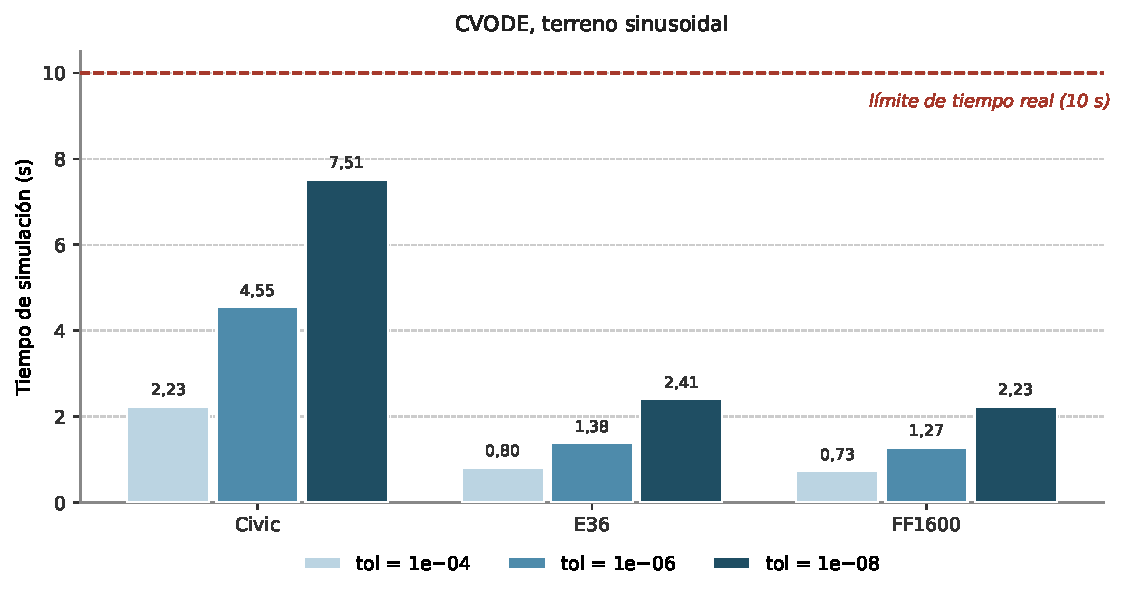
\includegraphics[width=0.86\textwidth]{img/tolerancia.pdf}
\caption[Costo en función de la tolerancia del integrador]{Tiempo de simulación con CVODE sobre terreno sinusoidal para tolerancias de $10^{-4}$, $10^{-6}$ y $10^{-8}$. La línea discontinua marca el límite de tiempo real: una barra que la supere indicaría que la simulación no puede sostener el ritmo del reloj. Ninguna configuración lo alcanza, ni siquiera con la tolerancia más estricta.}
\label{fig:tolerancia}
\end{figure}

El costo crece de forma regular: cada dos órdenes de magnitud de tolerancia adicional, se multiplica el tiempo de cómputo por un factor de entre $1{,}7$ y $2{,}0$.  \\

Comparando contra el tiempo real, incluso utilizando la tolerancia más estricta se preserva el margen: la relación contra el reloj con $10^{-8}$ es de $1{,}3\times$ para el Civic y $4{,}5\times$ para el FF1600, contra $12{,}4\times$ y $13{,}7\times$ respectivamente con $10^{-4}$. La elección de la tolerancia $10^{-6}$ para el resto de los experimentos se dio debido a que es un punto medio: conserva un buen margen contra el tiempo real, permitiendo más overhead para incluir carga adicional proveniente del resto del entorno, manteniendo un nivel de tolerancia aceptable. \\

% Vale la pena aclarar la falla del modelo E36 con $10^{-8}$, ya que es diferente a las fallas vistas anteriormente de DASSL. El error indica que el número de iteraciones del evento superó el límite establecido por default (veinte), lo que sugiere un encadenamiento de eventos que no llegan a converger (\textit{chattering}) y no una divergencia de la integración. Esto es debido a que al exigir mayor exactitud, el solver coloca los cruces por cero con más precisión, y detecta conmutaciones que con tolerancias mayores quedaban enmascaradas dentro del error admitido. Este límite es configurable mediante el indicador de tiempo de ejecución \verb|-mei=<valor>|, pero aumentar ese valor no resolvería la causa original, la mejor forma de solucionar esto es encontrar cuál es la conmutación responsable y suavizarla, del mismo modo que se hizo con la regulación a la resistencia a la rodadura, o con los frenos, descrito en la sección~\ref{sec:method}.


\subsection{Exactitud de la solución}

La sección anterior se dedicó a mostrar lo que cuesta aumentar la tolerancia, todavía queda por determinar cuanto se gana con ello. Para medirlo, se comparó con cada modelo, la trayectoria obtenida con diferentes tolerancias contra la tolerancia más escrita que se pudo correr en el modelo, para tomarla como referencia. 

El experimento se realizó de forma diferente al protocolo utilizado anteriormente, las principales diferencias fueron:

Las ejecuciones se realizaron sobre los FMU mediante la biblioteca \verb|fmpy| y no sobre el ejecutable de OpenModelica. La justificación es que el FMU admite tolerancias más estrictas. Utilizando esta metodología los tres vehículos pueden ejecutarse hasta  $10^{-10}$, valor que se toma como referencia. 

Los inputs de la simulación fueron reemplazados por una maniobra suave (dirección $0{,}2$ y acelerador $0{,}3$ constantes, sin frenada) en lugar de la maniobra extrema del benchmark de costo. Esto se realizó debido a que, utilizando los inputs anteriores, el neumático opera en el límite (y superando) de fricción, lugar donde las trayectorias vecinas divergen. Por lo tanto, utilizar la maniobra agresiva sirve para medir la divergencia del sistema, pero no es la mejor forma de medir la exactitud del integrador. Además, al ser una maniobra menos extrema, el tiempo de cómputo es menor, por lo que esta métrica no es directamente comparable con los de la tabla~\ref{tab:tolerancia}, que corresponden a otra maniobra y otro terreno.

Por último, todas las corridas se interpolan sobre una grilla temporal común. Fijar el intervalo de ejecución no es suficiente, porque \verb|fmpy| agrega una muestra por cada evento y el número de estos (y por lo tanto de entradas) varía según la tolerancia especificada. Los instantes de la grilla utilizada están presentes en los datos originales, de forma que la interpolación no introduce error de remuestreo.

Las medidas utilizadas para medir el error de la trayectoria son: el error de posición del chasis al final del intervalo de simulación $\lVert \mathbf{r}(T) - \mathbf{r}_\text{ref}(T) \rVert$, y el error cuadrático medio sobre toda la trayectoria normalizado por el desplazamiento total del vehículo (NRMSE), que hace comparables vehículos que recorrer distancias distintas. La Tabla~\ref{tab:exactitud} reúne los resultados y la Figura~\ref{fig:errorposicion} los representa.

\begin{table}[H]
\centering
\begin{tabular}{llccc}
\hline
Modelo & Tolerancia & Error final (m) & NRMSE (\%) & Razón de mejora \\
\hline
\multirow{3}{*}{FF1600}
 & $10^{-4}$ & $1{,}85\times10^{-2}$ & $1{,}8\times10^{-2}$ & --- \\
 & $10^{-6}$ & $4{,}68\times10^{-5}$ & $4{,}7\times10^{-5}$ & $395$ \\
 & $10^{-8}$ & $7{,}59\times10^{-7}$ & $<10^{-5}$ & $62$ \\
\hline
\multirow{3}{*}{E36}
 & $10^{-4}$ & $1{,}44\times10^{-2}$ & $9{,}4\times10^{-3}$ & --- \\
 & $10^{-6}$ & $2{,}30\times10^{-4}$ & $2{,}2\times10^{-4}$ & $63$ \\
 & $10^{-8}$ & $2{,}26\times10^{-6}$ & $<10^{-5}$ & $102$ \\
\hline
\multirow{3}{*}{Civic}
 & $10^{-4}$ & $2{,}25\times10^{-2}$ & $1{,}8\times10^{-2}$ & --- \\
 & $10^{-6}$ & $2{,}75\times10^{-4}$ & $1{,}7\times10^{-4}$ & $82$ \\
 & $10^{-8}$ & $1{,}12\times10^{-6}$ & $<10^{-5}$ & $245$ \\
\hline
\end{tabular}
\caption[Exactitud de la solución en función de la tolerancia]{Error respecto de la solución de referencia, calculada con tolerancia $10^{-10}$, para una maniobra suave de $10$ s. La razón de mejora es el cociente entre el error de la fila anterior y el de la fila actual. Los desplazamientos totales recorridos son de $42{,}9$ m (FF1600), $48{,}9$ m (E36) y $50{,}0$ m (Civic).}
\label{tab:exactitud}
\end{table}

\begin{figure}[H]
\centering
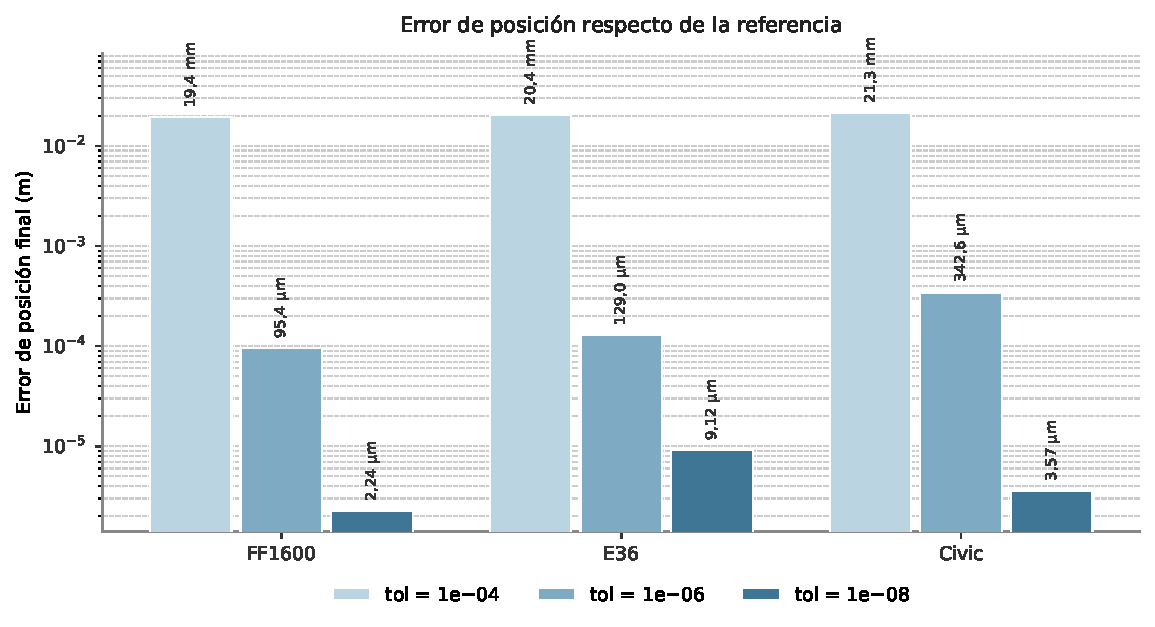
\includegraphics[width=0.86\textwidth]{img/error_posicion.pdf}
\caption[Error de posición en función de la tolerancia]{Error de posición del chasis al cabo de $10$ s respecto de la solución de referencia con tolerancia $10^{-10}$, en escala logarítmica. Sobre cada barra se indica el valor en unidades legibles.}
\label{fig:errorposicion}
\end{figure}

El comportamiento es el esperado, cada dos décadas de tolerancia el error se reduce aproximadamente dos órdenes de magnitud. Esta convergencia regular es evidencia de que la integración se comporta correctamente sobre este modelo.

En términos absolutos, las cifras son aceptables para el objetivo del simulador. Con la tolerancia $10^{-6}$ elegida, el error de posición al cabo de diez segundos de simulación es de $47$ a $275$ micrómetros sobre recorridos de unos cincuenta metros, equivalente un NRMSE inferior al $0{,}0002\text{\%}$. Incluso con la tolerancia más baja ensayada, $10^{-4}$, el apartamiento máximo es de $2{,}3$ cm, un valor que es imperceptible para un conductor e inferior a la incertidumbre de los propios parámetros del modelo (masas, rigideces y coeficientes de fricción) que se conocen con una precisión mucho menor. La tolerancia deja de ser el factor limitante de la fidelidad del simulador y en mi opinión pasaría a ser, por un lado, el conocimiento con mayor exactitud de las características del vehículo y por otro, una mayor fidelidad a la hora de plasmar ciertos aspectos de este, por ejemplo, eliminando la abstracción del chasis como un paralelepípedo e intercambiándola por algo más preciso.

Vale la pena mencionar que en casi todos los casos el error máximo sobre la trayectoria coincide con el error del final, lo que indica que este crece de forma monótona a lo largo de la maniobra, mostrando de que es un error acumulativo por truncamiento.



% Por último, una limitación del método: la referencia se obtiene con el mismo integrador que las soluciones evaluadas, de modo que lo que se mide es la \textit{convergencia} del esquema al refinar la tolerancia y no su exactitud frente a un método independiente. Un error sistemático común a todas las tolerancias no sería detectado por esta prueba. Una verificación cruzada exigiría contrastar contra DASSL sobre terreno plano, el único escenario en el que ese integrador resulta estable.

\subsection{Comparación de integradores}

Las mediciones de exactitud de la sección anterior compara CVODE contra sí mismo, por lo que mide la convergencia del sistema al modificar la tolerancia, pero no detectaría si hubiera un error común en el solver, independientemente de los parámetros. Esta sección agrega la verificación cruzada con otros solvers, comparando tres diferentes sobre el mismo modelo y maniobra.

Los integradores utilizados fueron: CVODE y DASSL, ambos de la familia de (BDF) y \verb|gbode|, de la familia de métodos Runge-Kutta de OpenModelica. Agregar el tercer método responde a una necesidad de agregar un solver que no comparta familia con los dos anteriores, para evitar ocultar errores posibles debido a la naturaleza de los sistemas, por lo que agregar un método de Runge-Kutta descarta esa posibilidad. 

Las ejecuciones se vuelven a correr como al principio de esta sección, utilizando el ejecutable de OpenModelica y no sobre el FMU. Esto es debido a dos razones, la primera es que \verb|fmpy| no ofrece ni DASSL ni \verb|gbode|, y la segunda es metodológica: comparar el CVODE de \verb|fmpy| contra el DASSL de OpenModelica agrega una segunda variable, el entorno de simulación, por lo que se decidió volver a realizar todo sobre un mismo entorno.


Se emplea la misma maniobra suave utilizada en la pureba de exactitud, por la misma razón que fue explicada en ese estudio. Las tolerancias son $10^{-4}$ y $10^{-6}$. Como OpenModelica escribe una grilla equidistante y el indicador \verb|-noEventEmit| suprime las muestras de evento, las mediciones caen exactamente sobre los mismos instantes, y por lo tanto no se requiere interpolación alguna. Cada configuración se repite tres veces para el tiempo de cómputo.


\begin{table}[H]
\centering
\begin{tabular}{llcc}
\hline
Modelo & Integrador & Tol. $10^{-4}$ & Tol. $10^{-6}$ \\
\hline
\multirow{3}{*}{FF1600}
 & CVODE & $0{,}49 \pm 0{,}02$ & $0{,}60 \pm 0{,}00$ \\
 & DASSL & falla$^{\S}$ & falla$^{\S}$ \\
 & gbode & $10{,}46 \pm 0{,}27$ & $12{,}97 \pm 0{,}34$ \\
\hline
\multirow{3}{*}{E36}
 & CVODE & $0{,}34 \pm 0{,}00$ & $0{,}38 \pm 0{,}00$ \\
 & DASSL & $0{,}38 \pm 0{,}00$ & $0{,}43 \pm 0{,}01$ \\
 & gbode & $4{,}98 \pm 0{,}14$ & $7{,}03 \pm 0{,}07$ \\
\hline
\multirow{3}{*}{Civic}
 & CVODE & $0{,}43 \pm 0{,}00$ & $0{,}53 \pm 0{,}00$ \\
 & DASSL & $0{,}48 \pm 0{,}01$ & $0{,}67 \pm 0{,}01$ \\
 & gbode & $1{,}30 \pm 0{,}01$ & $2{,}22 \pm 0{,}00$ \\
\hline
\end{tabular}
\caption[Tiempo de cómputo de los tres integradores]{Tiempo de cómputo en segundos (media $\pm$ desviación estándar de tres repeticiones) para la maniobra suave de $10$ s. $^{\S}$ Aborta a los $0{,}29$ s.}
\label{tab:solvers}
\end{table}

CVODE sigue siendo el solver más rápido en todas las configuraciones que completa:  DASSL cuesta entre $1{,}1$ y $1{,}3$ veces más, y \verb|gbode| entre $3$ y $22$ veces más. La diferencia era esperable en el caso de \verb|gbode|, cuyos métodos Runge-Kutta implícitos resuelven varios sistemas no lineales por paso.

Sigue habiendo una diferencia de robustez más marcada que de costo, pero concentrada en un único modelo, CVODE y \verb|gbode| completan todas las configuraciones, DASSL, sin embargo, falla en ambas pruebas del monoplaza.

% La brecha de robustez sigue siendo más marcada que la de costo, pero se concentra en un único modelo. CVODE y \verb|gbode| completan las seis configuraciones cada uno; DASSL falla en dos, ambas del monoplaza y con las dos tolerancias ensayadas. El aborto se produce a los $0{,}29$ s, durante el transitorio de asentamiento inicial y no en régimen establecido, lo que sugiere que la dificultad está en la fase en que la suspensión recorre su rango completo antes de estabilizarse. El diagnóstico es el mismo de siempre, \textit{«linear system solver failed»}, y no depende de la tolerancia, lo que descarta que se trate de un problema de control de error.

% Sin embargo, la diferencia más grande está en la robustez,  CVODE completa las seis configuraciones; \verb|gbode| falla en una; DASSL falla en dos, ambas del modelo E36 y con las dos tolerancias ensayadas. Es notable remarcar que DASSL aborta en el E36 incluso con la maniobra suave, cuando en el benchmark de costo solo fallaba sobre terreno sinusoidal, su fragilidad sobre este modelo no se limita a los regímenes de saturación.

La tabla~\ref{tab:acuerdo} y la figura~\ref{fig:acuerdo} presentan la diferencia entre pares de integradores con tolerancia $10^{-6}$, junto con el error propio de CVODE contra si mismo utilizando una tolerancia de $10^{-10}$, que sirve de comparación.

\begin{table}[H]
\centering
\begin{tabular}{lccc|c}
\hline
Modelo & CVODE--DASSL & CVODE--gbode & DASSL--gbode & Error propio de CVODE \\
\hline
FF1600 & ---       & $10{,}8$  & ---       & $46{,}8$  \\
E36    & $67{,}9$  & $87{,}6$  & $135{,}4$ & $229{,}6$ \\
Civic  & $95{,}2$  & $72{,}2$  & $164{,}3$ & $274{,}8$ \\
\hline
\end{tabular}
\caption[Diferencia entre integradores]{Diferencia de posición final entre pares de integradores, en micrómetros, con tolerancia $10^{-6}$. La última columna es el error de CVODE respecto de su propia referencia $10^{-10}$ (Tabla~\ref{tab:exactitud}). Los pares en que se usa DASSL no se informan para el monoplaza, porque ese integrador aborta sobre ese modelo.}
\label{tab:acuerdo}
\end{table}

\begin{figure}[H]
\centering
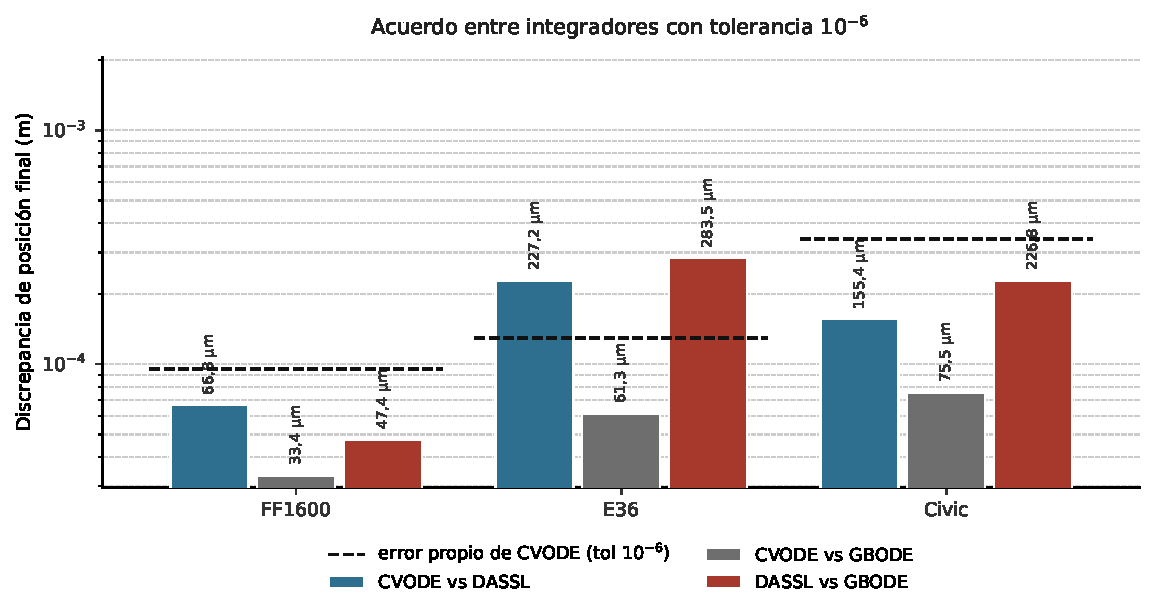
\includegraphics[width=0.86\textwidth]{img/solvers_acuerdo.pdf}
\caption[Acuerdo entre integradores]{Diferencia de posición final entre pares de integradores con tolerancia $10^{-6}$, en escala logarítmica. La línea discontinua marca, para cada vehículo, el error propio de CVODE a esa tolerancia: las diferencias del mismo orden indican acuerdo dentro de la exactitud alcanzable.}
\label{fig:acuerdo}
\end{figure}

El resultado es el buscado. Las diferencias entre pares de solver van de  $10{,}8$ a $164{,}3$ micrómetros, es decir, el mismo orden de magnitud que el error propio de CVODE frente a su referencia, de $46{,}8$ a $274{,}8$ micrómetros. Los tres métodos coinciden dentro de la exactitud que cada uno alcanza a esa tolerancia, no se detecta ningún sesgo generado por algún integrador en particular. Y dado que \verb|gbode| pertenece a otra familia de métodos, la coincidencia no puede explicarse por un problema compartido de la formulación BDF.

Con la tolerancia en $10^{-4}$ las diferencias crecen dos órdenes de magnitud, hasta $23{,}6$ mm, lo que también es consistente ya que el error propio de cada método es mayor de todas forams. El acuerdo entre integradores empeora en la misma proporción que la exactitud individual.

% La excepción vuelve a ser el modelo E36, que no admite verificación cruzada porque es el único que ningún otro integrador puede hacer que complete correctamente. El encadenamiento de eventos con tolerancias bajas refuerza de que puede ser un problema del modelo en sí y no del integrador. Queda pendiente identificar la conmutación responsable, probablemente en los topes de suspensión de la topología \verb|MultiLink|, queda como trabajo pendiente.


\subsection{Discusión}

\subsubsection{Robustez antes que velocidad}



% El hallazgo más significativo de este capítulo no es de rendimiento, si no de robustez. En el benchmark de costo DASSL aborta en cuatro de seis configuraciones, en la comparación de integradores falla en dos de seis y \verb|gbode| en una. CVODE, sin embargo, completa las doce configuraciones ejecutadas en ambos experimentos sin una sola falla.

Lo habitual al elegir un integrador es negociar entre velocidad y robustez. Sin embargo en este caso, CVODE es al mismo tiempo el más rápido (entre $1{,}1$ y $1{,}3$ veces más que DASSL, y entre $3$ y $22$ veces más que \verb|gbode|) y el único que no presenta fallas en las ejecuciones. Por lo tanto, la elección resulta sencilla y CVODE se adopta como integrador de referencia de la biblioteca.

\subsubsection{La tolerancia dejó de ser el factor limitante}

Los resultados de las pruebas de costo y exactitud proveen un resultado claro con respecto al ajuste de la tolerancia. Por el lado del costo, cada dos décadas de tolerancia agregada se duplica el tiempo de cómputo. Por el lado de la exactitud, estas mismas dos décadas reducen el error en dos órdenes de magnitud. El intercambio es favorable a ajustar la tolerancia y no existe razón de rendimiento para relajarla demasiado.
 
La medición mas relevante para observar es la magnitud absoluta del error. Con la tolerancia elegida de $10^{-6}$ la trayectoria se aparta de la referencia entre $47$ y $275$ micrómetros al cabo de diez segundos de simulación en el entorno ejecutado, e incluso con la tolerancia más permisiva, el error máximo es de $2{,}3$ cm. Ambas cifras son órdenes de magnitud menores que la incertidumbre con las que se conocen los parámetros físicos del modelo (masas, rigideces, coeficientes de fricción, geometría de la suspensión). El esfuerzo de mejora, rinde mucho más si es aplicado a la caracterización del vehículo antes que al control del error del integrador.

\subsubsection{Las conmutaciones son la dificultad numérica dominante}

Hay un patrón que se repite en todos los experimentos realizados: la dificultad numérica observada se atribuye a una no linealidad conmutativa y no al tamaño del sistema ni a la complejidad cinemática.

Se observó que la saturación del círculo de fricción degrada la convergencia de un factor $41$ a un factor $3{,}3$, haciendo que se invalide la maniobra agresiva para la prueba de exactitud.

La lección aprendida con estas pruebas es que rinde más invertir esfuerzo en suavizar de forma controlada las conmutaciones antes que ajustar los parámetros del integrador. Una discontinuidad que se encuentra en una condición de operación habitual puede costar más que el resto del modelo.



\subsubsection{Costo del terreno irregular}

Para CVODE, pasar de terreno plano al de la forma sinusoidal multiplica el tiempo de simulación por factores de entre $1{,}9$ (FF1600) y $5{,}4$ (Civic). Esto es consistente con lo esperado del modelo de contacto, sobre superficie plana la penetración del neumático se estabiliza en un valor casi constante, mientras que en el perfil sinusoidal oscila de forma continua, obligando al integrador a reducir el paso. Un detalle a tener en cuenta es que este terreno es una exageración de lo que se puede ver en la vida real, por lo que se debe tomar como un caso del peor escenario posible.

\subsubsection{Costo de inicialización}

La diferencia entre el tiempo total y el de simulación se puede usar para comparar el costo fijo de inicialización y escritura de resultados. Para CVODE se sitúa entre $0{,}034$ y $0{,}090$ s, mientras que para DASSL alcanza aproximadamente $0{,}32$ s. Este costo es irrelevante para estas pruebas ya que es una simulación por lotes, pero para el caso de tiempo real se puede ver como un retraso antes de comenzar la simulación interactiva, sin embargo, ambos son tiempos de espera asumibles.


\subsubsection{Complejidad del modelo y costo}

Contrastando los tiempos contra la tabla~\ref{tab:complejidad} se pueden observar dos efectos separados. El primero responde al tamaño del modelo: el E36 tiene $19{,}3\text{\%}$ menos de ecuaciones comparado a los otros vehículos (debido a su suspensión \verb|McPherson|, construida sobre una única articulación \verb|Prismatic| para simplificar) y es el más rápido de ejecutar sobre terreno plano.\\

El segundo efecto no se puede explicar de la misma forma. Los modelos \verb|Car| y \verb|CivicEKCar| tienen el mismo número de ecuaciones ($10\,981$), el mismo número de estados ($30$) y la misma topología de suspensión en las cuatro esquinas, pero sobre terreno sinusoidal el Civic tarda $2{,}85$ veces más que el FF1600. Dado que el tamaño del sistema es fijo, esa diferencia solo puede provenir del número de pasos que el integrador necesitar dar debido a la rigidez numérica que introducen los parámatros utilizados en el modelo. La masa suspendida, la rigidez del muelle y el amortiguamiento determinan la frecuencia del conjunto y en consecuencia el paso máximo admisible. El Civic, con $990$ kg de masa suspendida sobre muelles de $16$ y $14$ kN/m, presenta una dinámica vertical más exigente de seguir que el monoplaza de $400$ kg.\\

La conclusión es que el costo de estos modelos tiene dos componentes independientes: el tamaño del sistema en sí y la rigidez de la dinámica, y que reducir el primero no reduce necesariamente el segundo.


\subsubsection{Qué limita realmente al simulador}

Reuniendo todo lo anterior, la capacidad de cómputo no es la restricción principal que tiene este simulador. Con márgenes de entre $2{,}4\times$ y $16{,}1\times$ respecto del tiempo real sobre la maniobra más exigente y con un error de integración de centésimas de milímetro, ni la velocidad ni la exactitud del integrador son los factores que pueden acatar la calidad del resultado.

Las principal restricción que posee el modelo es su robustez, un modelo puede resultar numéricamente frágil con independencia del margen de cómputo disponible.

Este margen extra se puede invertir, en las pruebas de lazo cerrado, parte de este se va a ir a la ejecución tanto de las interfaces como de el entorno gráfico. Sin embargo, el margen es lo suficientemente grande como para agregar modelos de neumático o de suspensión más detallados, o la simulación simultánea de varios vehículos sin comprometer la operación interactiva.


% \subsection*{Limitaciones de la medición}

% Los tiempos del \textit{benchmark} de costo —Tablas~\ref{tab:tiempos} y \ref{tab:tolerancia}— corresponden a una única ejecución por configuración, sin repeticiones, por lo que no se dispone de una estimación de su dispersión. El estudio de exactitud sí repite cinco veces cada configuración, con desviaciones estándar de entre $0{,}01$ y $0{,}13$ s, lo que da una idea del orden de la variabilidad esperable también en aquellas mediciones. En una máquina de propósito general, con planificación de procesos y estados de caché variables, la variabilidad entre corridas idénticas puede ser significativa. Las conclusiones cualitativas —el orden de magnitud del margen respecto del tiempo real, y sobre todo el patrón de fallas de DASSL, que es determinista— son robustas frente a esa incertidumbre; las comparaciones finas entre vehículos, en cambio, deberían respaldarse con la media y la desviación estándar sobre un número suficiente de repeticiones.

% Debe señalarse además que un valor medio de tiempo por paso, aun holgadamente inferior al umbral de tiempo real, no garantiza por sí solo una experiencia interactiva satisfactoria: lo que percibe el conductor es el peor caso, no el promedio.


\section{Simulación a lazo cerrado}

Todas las mediciones anteriores son simulaciones por lotes, el modelo se ejecuta con una maniobra predefinida y se observan los resultados luego de que esta termina. En esta sección se va a medir el sistema completo en funcionamiento, con el volante y pedales físicos generando comandos al vehículo y el visualizador de Unity recibiendo las poses. Esta medición va a caracterizar al simulador tal y como lo experimenta un conductor humano.

\subsection{Montaje}

La aplicación de control descrita en la sección~\ref{sec:method} se encarga de recibir los comandos en el puerto $12344$, avanza la integración en un paso de $10$ ms (por defecto), convierte las matrices de rotación a cuaterniones y emite las cinco poses (chasis y cuatro ruedas) a los puertos $12345$ a $12349$. La tolerancia es $10^{-6}$ y la sincronización con el reloj de tiempo real está activa. Se registraron los resultados durante $45$ segundos de conducción en cada uno de los vehículos desarrollados.

La medición de mayor interés es la \textbf{latencia entrada$\rightarrow$pose}, que es el intervalo entre la llegada del datagrama del comando del conductor y la emisión de la pose calculada a partir de él. Debe notarse que esta latencia no es la que percibe el conductor, queda omitida la latencia de adquisición del propio periférico, el trayecto por la red y el renderizado en Unity.

También se registran el tiempo de integración por paso, el período efectivo del bucle, la antigüedad del comando al momento de aplicarse y la separación entre datagramas de entrada.

Para separar el costo propio del modelo del que introduce la interacción, cada configuración se repitió con el puerto de entrada muerto, sin recibir datagramas. Unity sigue ejecutándose y el resto del montaje no cambia, de modo que la única diferencia es que los inputs son constantes.


\paragraph{Resultados.} La Tabla~\ref{tab:lazo} y las Figuras~\ref{fig:latencialazo} y~\ref{fig:pasolazo} reúnen las mediciones.

\begin{table}[H]
\centering
\begin{tabular}{lccc|ccc|cc}
\hline
 & \multicolumn{3}{c}{Latencia entrada$\rightarrow$pose} & \multicolumn{3}{c}{Integración por paso} & \multicolumn{2}{c}{Pasos $>10$ ms} \\
Vehículo & p50 & p95 & p99 & p50 & p95 & p99 & viva & const. \\
\hline
FF1600 & $15{,}1$ & $22{,}0$ & $27{,}1$ & $6{,}69$ & $14{,}28$ & $18{,}72$ & $29{,}0\%$ & $0{,}03\%$ \\
E36    & $13{,}1$ & $18{,}4$ & $26{,}5$ & $3{,}81$ & $9{,}49$  & $14{,}11$ & $3{,}8\%$  & $0{,}03\%$ \\
Civic  & $15{,}6$ & $24{,}3$ & $30{,}7$ & $7{,}24$ & $16{,}30$ & $21{,}64$ & $34{,}9\%$ & $0{,}03\%$ \\
\hline
\end{tabular}
\caption[Perfil del lazo cerrado en tiempo real]{Percentiles en milisegundos medidos sobre $45$ s de conducción real con cada vehículo, con paso de comunicación de $10$ ms y tolerancia $10^{-6}$. Las dos últimas columnas indican la fracción de pasos cuya integración excede el presupuesto de $10$ ms, con entrada viva y con la entrada constante de la condición de control.}
\label{tab:lazo}
\end{table}

\begin{figure}[H]
\centering
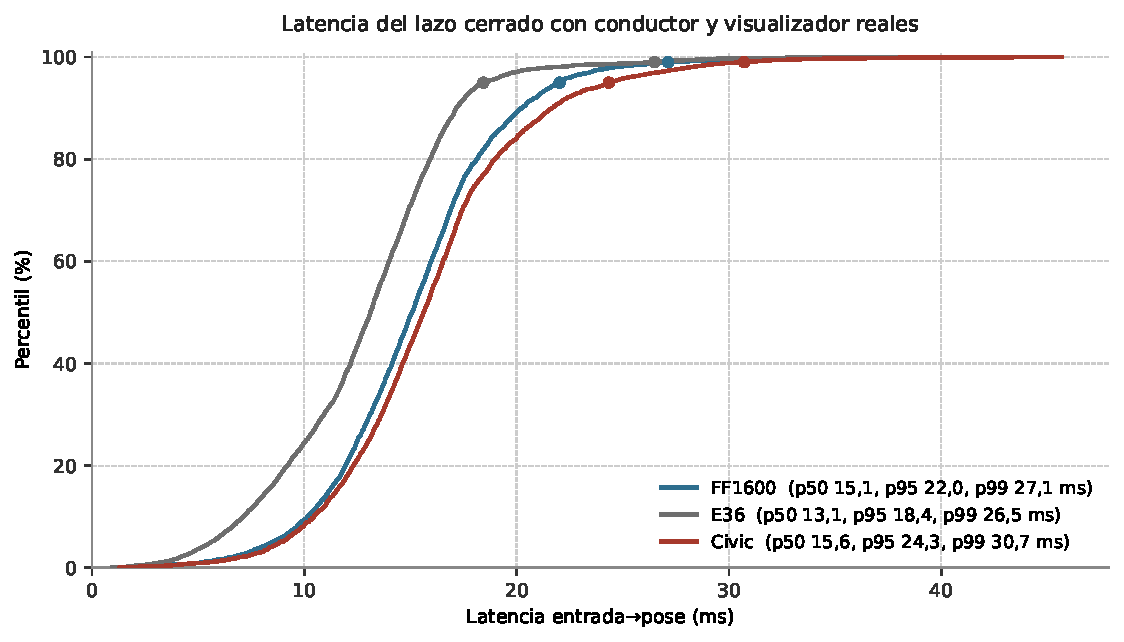
\includegraphics[width=0.86\textwidth]{img/latencia_lazo.pdf}
\caption[Distribución de la latencia del lazo cerrado]{Distribución acumulada de la latencia entrada$\rightarrow$pose para los tres vehículos. Los puntos marcan los percentiles $95$ y $99$. La mediana se sitúa entre $13$ y $16$ ms y la cola no supera los $31$ ms en el percentil $99$.}
\label{fig:latencialazo}
\end{figure}

\begin{figure}[H]
\centering
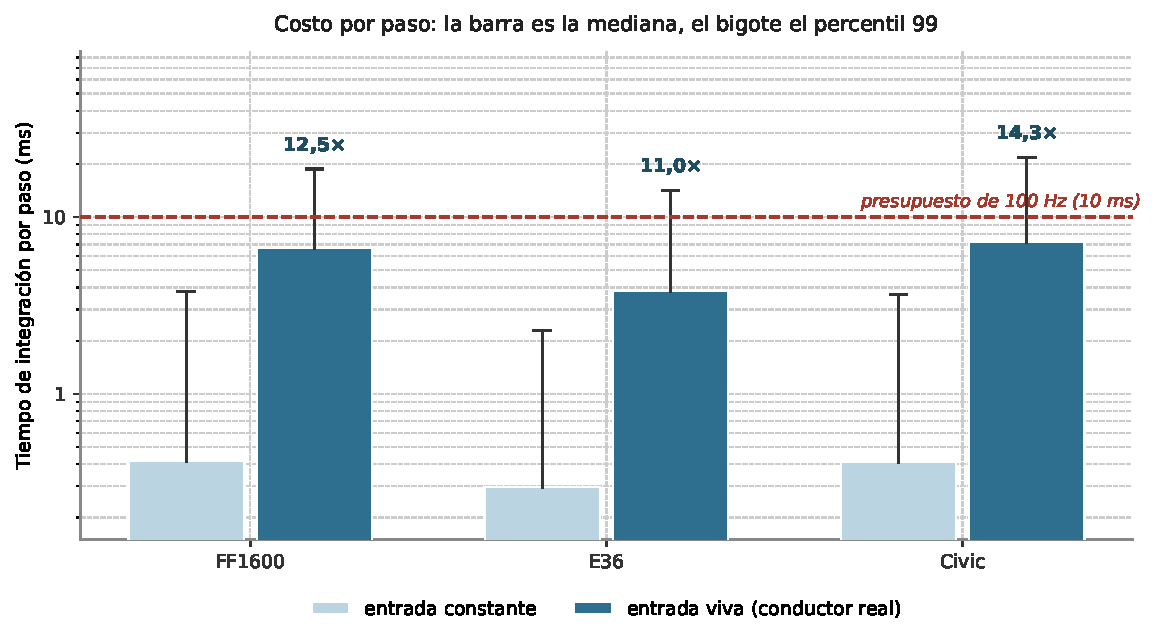
\includegraphics[width=0.86\textwidth]{img/paso_lazo.pdf}
\caption[Costo por paso con entrada viva y constante]{Tiempo de integración por paso en escala logarítmica. La barra es la mediana y la línea superior alcanza el percentil $99$. La línea discontinua marca el presupuesto de $10$ ms del paso de comunicación.}
\label{fig:pasolazo}
\end{figure}

Las nueve corridas completan su horizonte con un factor de $1{,}00\times$ respecto del reloj de tiempo real y sin descartar una sola pose. Se emitieron entre $22\,500$ y $22\,700$ datagramas por corrida, cinco por paso. La sincronización se mantiene con un período mediano de $10{,}07$ ms frente a los $10$ ms nominales.

Con medianas de $13$ a $16$ ms y percentiles $99$ de $26$ a $31$ ms, la contribución del modelo equivale a entre una y dos tramas a $60$ Hz. La antigüedad mediana del comando al aplicarse es de $7{,}6$ ms, mientras que la integración mediana cuesta entre $3{,}8$ y $7{,}2$ ms. Es decir aproximadente la mitad de la latencia no viene de la simulación si no de la espera del comando, sin embargo, siguen siendo valores bajos e imperceptibles para el humano.

Esta espera viene de la frecuencia de actualización del periférico. La separación mediana entre datagramas de comandos es de $15{,}60$ ms, equivalente a $64{,}1$ Hz, y no a los $100$ Hz que la aplicación de control asume. Elevar esta frecuencia reduciría el término dominante de la latencia. Un detalle a tener en cuenta es que la base utilizada en estas pruebas reporta una frecuencia de $1000$ Hz, por lo que esa limitante probablemente venga de la implementación de \textit{DeviceDrivers}.

Con la entrada constante, la integración cuesta entre $0{,}30$ y $0{,}42$ ms por paso, con el conductor real, entre $3{,}81$ y $7{,}24$ ms. El factor es de $11{,}0$ a $14{,}3$ según el vehículo. La causa de esto es la variación generada por la entrada: cada actualización del comando introduce un escalón en la señal mantenida, y con actualizaciones cada $15{,}6$ ms, prácticamente todo paso arrastra una perturbación que obliga al integrador a reducir el paso interno para recuperar la exactitud.

La consecuencia de esto es que las mediciones de lazo abierto obtenidas anteriormente, y particularmente los márgenes de $2{,}4\times$ a $16{,}1\times$ de la figura~\ref{fig:tiemporeal} son correctos para lo que miden, pero su comparación no es directa con la operación interactiva.


% \paragraph{La media no es la magnitud que importa.} Entre el $3{,}8\,\%$ y el $34{,}9\,\%$ de los pasos exceden el presupuesto de $10$ ms y, sin embargo, el lazo sostiene $1{,}00\times$ el tiempo real. La aparente contradicción se explica porque el acompasamiento solo espera cuando hay holgura: un paso de $16$ ms se compensa con los siguientes, que no duermen. En promedio el presupuesto se cumple; instante a instante, no. Contra la condición de control, donde apenas un paso de tres mil excede el presupuesto, queda claro que la ocupación pasa de un $4\,\%$ a un rango del $38$ al $72\,\%$ al cerrar el lazo con un conductor real. La holgura sigue existiendo, pero es un factor y no un orden de magnitud.

La extracción de las cinco poses y su conversión a cuaternión consumen entre $0{,}14$ y $0{,}20$ ms por paso, esto es, del $2$ al $3\%$ del total. La elección de Python para la aplicación de control no penaliza demasiado, la totalidad del costo reside en la integración, que ocurre en el código compilado de SUNDIALS.


\subsection{Limitaciones de esta medición} 
La conducción no fue guionada, los tres vehículos no se condujeron de forma idéntica, aunque se intentó mantener un comportamiento similar, por lo que las comparaciones entre ellos son indicativas y no controladas.


% \subsection*{Discusión}

% \paragraph{Robustez antes que velocidad.} El hallazgo más significativo de todo el capítulo no es de rendimiento sino de robustez, y los dos experimentos independientes coinciden en él. En el \textit{benchmark} de costo DASSL aborta en cuatro de seis configuraciones, incluida la totalidad de las que emplean terreno irregular; en la comparación de integradores aborta en dos de seis, y \verb|gbode| en una. CVODE, en cambio, completa las doce configuraciones de ambos experimentos sin una sola falla.

% Lo habitual al elegir un integrador es negociar entre velocidad y robustez. Aquí no hay tal negociación: CVODE es simultáneamente el más rápido —entre $1{,}5$ y $2{,}2$ veces más que DASSL, y entre $4$ y $6$ veces más que \verb|gbode|— y el único que nunca falla. La elección resulta, por lo tanto, inusualmente sencilla, y CVODE se adopta como integrador de referencia de la biblioteca.

% \paragraph{La tolerancia dejó de ser el factor limitante.} Los resultados de costo y de exactitud, leídos en conjunto, dan una respuesta clara al ajuste de la tolerancia. Del lado del costo, cada dos décadas de tolerancia adicional cuestan aproximadamente el doble de tiempo de cómputo. Del lado de la exactitud, esas mismas dos décadas reducen el error unos dos órdenes de magnitud. El intercambio es, por lo tanto, muy favorable a ajustar la tolerancia, y no existe razón de rendimiento para relajarla.

% Más relevante aún es la magnitud absoluta del error. Con la tolerancia $10^{-6}$ adoptada, la trayectoria se aparta de la de referencia entre $119$ y $233$ micrómetros al cabo de diez segundos de conducción, e incluso con la tolerancia más laxa ensayada el apartamiento máximo es de $2{,}1$ cm. Ambas cifras son varios órdenes de magnitud menores que la incertidumbre con la que se conocen los parámetros físicos del modelo —masas, rigideces, coeficientes de fricción, geometría de la suspensión—, que son en última instancia quienes acotan la fidelidad del simulador. El esfuerzo de mejora, por lo tanto, rinde mucho más aplicado a la caracterización del vehículo que al control de error del integrador.

% \paragraph{Las conmutaciones son la dificultad numérica dominante.} Un patrón atraviesa todos los experimentos de este capítulo: cada dificultad numérica observada se remonta a una no linealidad conmutativa, y ninguna al tamaño del sistema ni a la complejidad cinemática.

% La saturación del círculo de fricción degrada la convergencia de un factor $41$ a un factor $3{,}3$, hasta el punto de invalidar la maniobra agresiva como base de un estudio de exactitud. El modelo E36 multiplica por siete el número de muestras que devuelve al relajar la tolerancia, señal de un encadenamiento de eventos que no converge, y es el mismo modelo que aborta con $10^{-8}$ por exceso de iteraciones de evento y el único que ningún integrador alternativo consigue integrar. Las tres manifestaciones son caras distintas de un mismo problema. Y, en sentido inverso, las dos leyes de fuerza incorporadas al modelo físico —resistencia aerodinámica y resistencia a la rodadura— solo resultaron numéricamente inocuas porque se regularizó explícitamente su comportamiento en el entorno del reposo.

% La manifestación más costosa de todas, sin embargo, no está en el modelo sino en su entrada. El escalón que introduce cada actualización del comando del conductor multiplica por entre $11$ y $14$ el costo de integración respecto de una entrada constante, según se estableció en la sección anterior. Es la misma clase de perturbación —una discontinuidad que el integrador debe absorber reduciendo el paso— y su efecto supera a cualquier otro medido en este capítulo. Suavizar la reconstrucción del comando, en lugar de mantenerlo constante entre actualizaciones, es por lo tanto la optimización de mayor rendimiento potencial que este trabajo deja identificada.

% La lección práctica, transferible a modelos de esta clase, es que el esfuerzo invertido en suavizar de forma controlada las conmutaciones rinde más que el invertido en ajustar los parámetros del integrador. Una discontinuidad situada justamente en la condición de operación habitual —el reposo, en el caso de la resistencia a la rodadura— puede costar más que todo el resto del modelo.

% \paragraph{Costo del terreno irregular.} Para CVODE, pasar de terreno plano a sinusoidal multiplica el tiempo de simulación por factores de entre $1{,}9$ (FF1600) y $5{,}4$ (Civic). Esto es consistente con la naturaleza del modelo de contacto: sobre superficie plana la penetración del neumático se estabiliza en un valor cuasi-constante tras el asentamiento inicial, mientras que sobre el perfil sinusoidal oscila de forma continua, obligando al integrador a reducir el paso para seguir la dinámica vertical de la suspensión.

% \paragraph{Costo de inicialización.} La diferencia entre el tiempo total y el de simulación mide el costo fijo de inicialización y escritura de resultados. Para CVODE se sitúa entre $0{,}034$ y $0{,}090$ s, mientras que para DASSL alcanza aproximadamente $0{,}32$ s en las corridas completas. Aunque irrelevante para una simulación por lotes, este costo fijo sí importa en el arranque de una sesión interactiva.

% \paragraph{Complejidad del modelo y costo.} Confrontando los tiempos con la Tabla~\ref{tab:complejidad} se distinguen dos efectos separados. El primero sí responde al tamaño del modelo: el E36 tiene un $21{,}6\,\%$ menos de ecuaciones que los otros dos vehículos —consecuencia de que la suspensión \verb|McPherson|, construida sobre una única articulación \verb|Prismatic|, es cinemáticamente mucho más simple que el bucle cerrado del doble triángulo— y es, coherentemente, el más rápido sobre terreno plano: evaluar el lado derecho del sistema le cuesta menos.\\

% El segundo efecto no admite esa explicación. Los modelos \verb|Car| y \verb|CivicEKCar| tienen el mismo número de ecuaciones ($10\,981$), el mismo número de estados ($30$) y la misma topología de suspensión en las cuatro esquinas; sin embargo, sobre terreno sinusoidal el Civic tarda $2{,}85$ veces más que el FF1600. Con el tamaño del sistema fijo, esa diferencia solo puede provenir del número de pasos que el integrador necesita dar, es decir, de la rigidez numérica que introduce la parametrización concreta de cada vehículo: la masa suspendida, la rigidez del muelle y el amortiguamiento determinan la frecuencia propia del conjunto y, con ella, el paso máximo admisible. El Civic, con $990$ kg de masa suspendida sobre muelles de $16$ y $14$ kN/m, presenta una dinámica vertical más exigente de seguir que el monoplaza de $400$ kg.\\

% La conclusión práctica es que el costo de estos modelos tiene dos componentes independientes —el tamaño del sistema y la rigidez de la dinámica— y que reducir el primero, por ejemplo simplificando la cinemática de la suspensión, no reduce necesariamente el segundo.

% \paragraph{Qué limita realmente al simulador.} La exactitud no es la restricción: con errores del orden de las centésimas de milímetro y muy por debajo de la incertidumbre de los parámetros, el control de error del integrador no acota la calidad del resultado. El presupuesto de cómputo, en cambio, resulta bastante más ajustado de lo que las mediciones por lotes sugieren.

% La medición del lazo cerrado obliga a matizar los márgenes holgados de la Figura~\ref{fig:tiemporeal}. Al cerrar el lazo con un conductor real, la ocupación del presupuesto de $10$ ms pasa de un $4\,\%$ —con entrada constante— a un rango del $38$ al $72\,\%$, y entre el $4$ y el $35\,\%$ de los pasos individuales lo exceden. La holgura sigue siendo real, pero es un factor de dos o tres y no el orden de magnitud que el \textit{benchmark} por lotes anticipaba. Un modelo de neumático o de suspensión sensiblemente más detallado ya no entraría sin más.

% Las dos restricciones que gobiernan son, por lo tanto, la dispersión del tiempo por paso —no su media, dado que el acompasamiento compensa los excesos aislados a costa de la regularidad instantánea— y la robustez del modelo. El caso del E36 ilustra la segunda con claridad: un modelo puede resultar numéricamente frágil, hasta el punto de que dos de los tres integradores no logren integrarlo, con total independencia del margen de cómputo disponible. Y resulta llamativo que sea justamente el E36, el más frágil de los tres, el que menos cuesta en el lazo cerrado.

% Queda además una restricción que este trabajo no llegó a medir: la latencia total tal como la percibe el conductor. La contribución del modelo y su acoplamiento, de $13$ a $16$ ms de mediana, está caracterizada; la del periférico y la del renderizado en Unity, no.

% \subsection*{Limitaciones de la medición}

% Los tiempos del \textit{benchmark} de costo —Tablas~\ref{tab:tiempos} y \ref{tab:tolerancia}— corresponden a una única ejecución por configuración, sin repeticiones, por lo que no se dispone de una estimación de su dispersión. El estudio de exactitud sí repite cinco veces cada configuración, con desviaciones estándar de entre $0{,}01$ y $0{,}13$ s, lo que da una idea del orden de la variabilidad esperable también en aquellas mediciones. En una máquina de propósito general, con planificación de procesos y estados de caché variables, la variabilidad entre corridas idénticas puede ser significativa. Las conclusiones cualitativas —el orden de magnitud del margen respecto del tiempo real, y sobre todo el patrón de fallas de DASSL, que es determinista— son robustas frente a esa incertidumbre; las comparaciones finas entre vehículos, en cambio, deberían respaldarse con la media y la desviación estándar sobre un número suficiente de repeticiones.

% La medición del lazo cerrado, en cambio, sí informa percentiles sobre varios miles de pasos, y confirma la advertencia que motivaba esta precaución: un valor medio de tiempo por paso holgadamente inferior al umbral de tiempo real no garantiza por sí solo una experiencia interactiva satisfactoria, puesto que entre el $4$ y el $35\,\%$ de los pasos individuales exceden el presupuesto pese a que el promedio lo cumple. Su principal limitación es de otro tipo: la conducción no fue guionada, de modo que las comparaciones entre vehículos de esa sección no están controladas.

\section{Fidelidad del manejo}

Todas las mediciones anteriores son de carácter numérico, cuánto cuesta la simulación, cuánto tardan los integradores en coincidir, y con qué exactitud converge son medidas útiles para comparar el performance del modelo y de los integradores, pero no dicen nada sobre si el resultado se comporta como un vehículo real. Esta sección se centra en responder esa cuestión, comparando cuatro magnitudes del modelo contra lo que predice la teoría de dinámica vehicular y los valores típicos de automóviles reales.

Estos cuatro ensayos se eligieron por ser medibles sin instrumentar el modelo y cubren los ejes de la dinámica vehicular: el vertical, el lateral y el longitudinal.

\subsection{Frecuencia propia de la suspensión}

La frecuencia de la suspensión en su translación vertical (\textit{ride frequency}) es la manera más directa de medir el comportamiento vertical de un vehículo ante diferentes perturbaciones.

% La frecuencia de la suspensión en su modo de traslación vertical (\textit{ride frequency}) es el descriptor más inmediato del comportamiento vertical de un vehículo: fija la sensación de firmeza y determina el ancho de banda de las perturbaciones del terreno que la carrocería sigue.


% El ensayo se realiza, por lo tanto, dejando asentar el vehículo y perturbando después el estado correspondiente, con acceso al vector de estados a través de la interfaz de bajo nivel del FMU descrita en la Sección~\ref{sec:cosim}. Sobre la respuesta resultante se identifica un sistema de segundo orden, $\ddot{e} = -a\,\dot{e} - b\,e$, cuyo ajuste es lineal en los coeficientes y no depende de localizar máximos —escasos en una respuesta amortiguada—, de donde $\omega_n = \sqrt{b}$ y $\zeta = a / (2\omega_n)$.

Para realizar este ensayo se perturbó el estado de velocidad vertical del chasis, haciendo esto, los neumáticos conservan su compresión y los resortes de su deflexión al inicio, y al aplicar el impulso se excitan de forma natural, haciendo que el chasis se desplace mientras las ruedas permaneces quietas. El impulso empleado es de $0{,}05$ m/s, que produce amplitudes de $1{,}7$ a $2{,}4$ mm.

Sobre el resultado se obtiene un sistema de segundo orden. Dado que es un sistema resorte-amortiguador la ecuación que lo describe es la siguiente (escrita para un desplazamiento $e$ respecto a la altura de equilibrio).

\begin{equation}
    \ddot{e} = -\frac{c}{m}\,\dot{e} \;-\; \frac{k}{m}\,e
    \label{eq:segundo-orden}
\end{equation}

donde $m$ es la masa suspendida, $k$ la rigidez vertical y $c$ el amortiguamiento. De estos datos se pueden obtener la frecuencia natural y el amortiguamiento relativo:

\begin{equation}
    f_n = \frac{1}{2\pi}\sqrt{\frac{k}{m}},
    \qquad
    \zeta = \frac{c/m}{2\sqrt{k/m}}
    \label{eq:fn-zeta}
\end{equation}

El valor $R^2$ es el coeficiente de determinación, que es una medida de comparación entre el resultado esperado según la fórmula y el real, particularmente compara las aceleraciones. Un número cercano a 1 de de este valor confirmaría que este sistema es efectivamente de segundo orden y que no hay factores externos que lo modifiquen.

% El ajuste es lineal en ambos cocientes, de modo que tiene solución cerrada y aprovecha todas las muestras en lugar de depender de localizar máximos, que en una respuesta amortiguada son escasos. Su coeficiente de determinación $R^2$ sirve además de control: la Ecuación~\ref{eq:segundo-orden} es una hipótesis sobre el comportamiento del vehículo, no un hecho, y el $R^2$ mide si un único par de cocientes explica efectivamente toda la respuesta registrada. De no ser así, la frecuencia identificada no significaría nada.

% La Figura~\ref{fig:ajuste} superpone, para cada vehículo, la respuesta medida sobre el modelo y la función de segundo orden así identificada. La coincidencia es estrecha en el primer ciclo, que es donde reside la información sobre la frecuencia, y se abre en el rebote posterior: el modelo identificado predice un retroceso por debajo del cero algo mayor que el que el vehículo realmente describe. Esa discrepancia es la que explica que el $R^2$ se sitúe en torno a $0{,}97$ y no en la unidad, y su origen es que el vehículo completo no es un oscilador de un grado de libertad sino que acopla el modo vertical con el de cabeceo. El E36 es el caso que mejor ajusta, con $R^2 = 0{,}987$, y también aquel en que ambas curvas resultan casi indistinguibles.

\begin{figure}[H]
\centering
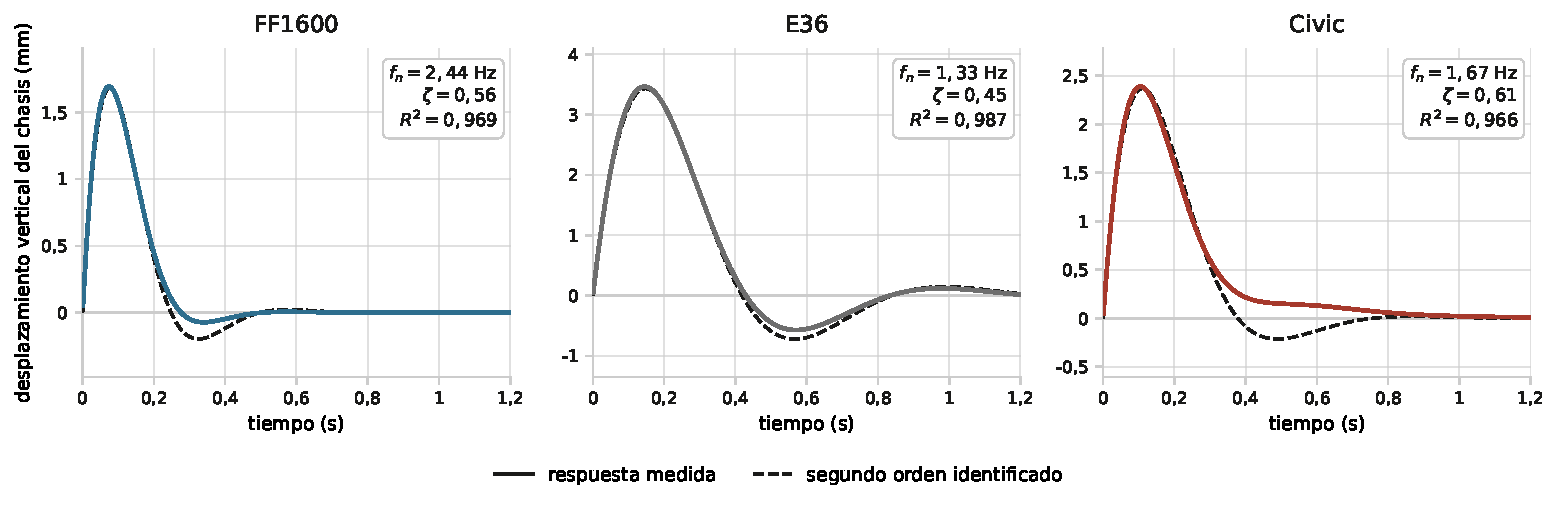
\includegraphics[width=\textwidth]{img/ajuste_segundo_orden.pdf}
\caption[Ajuste de segundo orden sobre la respuesta vertical]{Respuesta vertical libre del chasis tras el impulso de velocidad de $0{,}05$ m/s, en trazo continuo, y función de segundo orden identificada sobre ella, en trazo discontinuo. Un panel por vehículo, con las escalas verticales ajustadas a cada caso. Notar que las amplitudes son de apenas unos milímetros.}
\label{fig:ajuste}
\end{figure}

\begin{table}[H]
\centering
\begin{tabular}{lccccc}
\hline
Modelo & $f_n$ medida (Hz) & $\zeta$ & $R^2$ & Predicción (Hz) & Vehículo real (Hz) \\
\hline
FF1600 & $2{,}44$ & $0{,}56$ & $0{,}969$ & $2{,}42$ & $1{,}5$--$2{,}0$ \\
E36    & $1{,}33$ & $0{,}45$ & $0{,}987$ & $1{,}24$ & $0{,}5$--$1{,}5$ \\
Civic  & $1{,}67$ & $0{,}61$ & $0{,}966$ & $1{,}16$ & $0{,}5$--$1{,}5$ \\
\hline
\end{tabular}
\caption[Frecuencia propia y amortiguamiento de la suspensión]{Frecuencia natural y amortiguamiento relativo del modo vertical de la masa suspendida, identificados sobre la respuesta libre a un impulso de velocidad de $0{,}05$ m/s desde el estado asentado. La predicción es la Ecuación~\ref{eq:fn-zeta} evaluada con la rigidez y la masa declaradas en el modelo en lugar de con los cocientes ajustados, esto es $\frac{1}{2\pi}\sqrt{k_\text{ef}/m_\text{susp}}$, tomando el resorte en serie con la rigidez del neumático. La última columna muestra el rango habitual del tipo de vehículo que cada modelo representa. \cite{giaraffa_springs1}}
\label{tab:ride}
\end{table}

El caso del monoplaza da confianza en el procedimiento, su frecuencia medida coincide con la predicción teórica, es decir, para este vehículo el modelo se comporta como predice la fórmula. Los coeficientes de determinación confirman además que el modo es de segundo orden en los tres casos.

% \paragraph{El ensayo se valida a sí mismo.} El caso del monoplaza es el que da confianza en el procedimiento: su frecuencia medida, $2{,}44$ Hz, coincide con la predicción teórica, $2{,}42$ Hz, dentro del $1\,\%$. Es decir que para este vehículo el modelo se comporta exactamente como predice la fórmula elemental, lo que verifica a la vez la excitación empleada, el procedimiento de identificación y la propia predicción. Los coeficientes de determinación, entre $0{,}97$ y $0{,}99$, confirman además que el modo es efectivamente de segundo orden en los tres casos.

El resultado más interesante es la comparación con vehículos reales, para la que se toman como referencia los rangos de frecuencia de suspensión habituales en la práctica de la dinámica vehicular \cite{giaraffa_springs1,milliken1995}. El E36 se encuentra dentro de los rangos característicos de un vehículo de calle. En el caso del FF1600, si bien queda por encima del valor real esperado, este número no se pudo verificar con exactitud, principalmente por el hecho de que en autos de competición, los reglajes varían mucho entre equipos y circuitos, y no se tiene una fuente certera. Lo relevante, es que se ubica por encima de un vehículo de calle y por debajo de uno de competición con carga aerodinámica fuerte (entre  $3{,}0$ a $5{,}0$ Hz \cite{giaraffa_springs1}), por lo que es un punto medio en el que un monoplaza de este estilo puede vivir.


% El FF1600 queda donde corresponde un monoplaza sin carga aerodinámica, más duro que un vehículo de calle pero no tanto como un auto de competición con apoyo aerodinámico. En ambos casos el ensayo muestra que el comportamiento vertical coincide con el vehículo real.

El Civic también queda por encima del rango que le correspondería y es el que más se aparta de su predicción teórica. Esto se debe a que la predicción supone que el resorte se comprime lo mismo que la rueda, pero este está montado sobre los brazos de la suspensión, por lo que el cociente entre ambos recorridos (relación de instalación) depende de donde se fijen sus extremos. Calculando ese cociente en el modelo resulta en que el resorte recorre un $24\%$ más que la rueda, cuando en un vehículo real recorre menos de lo que recorre la rueda. Corregir los puntos de anclaje del conjunto resorte-amortiguador, llevándolos a una posición correspondiente al vehículo real ayudaría a que el modelo tenga valores más cercanos a la realidad, sin necesidad de tocar las rigideces declaradas.

% El Civic, con $1{,}67$ Hz, es el único que queda por encima del rango que le correspondería, y también el que más se aparta de su predicción teórica. Ambas desviaciones tienen la misma causa. La predicción supone que el resorte se comprime lo mismo que sube la rueda, pero el resorte no está montado sobre la rueda sino sobre los brazos de la suspensión, de modo que el cociente entre ambos recorridos —la \textit{relación de instalación}— depende de dónde se fijen sus extremos. En el Civic ese cociente vale $1{,}24$: el resorte recorre un $24\,\%$ más que la rueda, cuando en un automóvil real recorre \emph{menos}, entre un $50$ y un $70\,\%$ de lo que recorre la rueda. Como la rigidez percibida en la rueda escala con el cuadrado de esa relación, el vehículo resulta alrededor de un $50\,\%$ más rígido de lo que sus resortes declaran, y su frecuencia sube en consecuencia. Corregir los puntos de anclaje del conjunto muelle-amortiguador, llevándolos a una posición representativa de un vehículo real, situaría al Civic dentro del rango de calle sin necesidad de retocar las rigideces declaradas, que son valores realistas. Los otros dos vehículos no presentan el problema: el eje delantero del E36 tiene una relación de instalación de $1$ por construcción, su eje trasero de $0{,}92$ y el monoplaza de $0{,}97$.

El amortiguamiento relativo supera en los tres casos el rango habitual de $0{,}2$ a $0{,}4$ de un vehículo de calle \cite{giaraffa_springs3}, lo que se traduciría en una respuesta vertical algo más apagada que la real. Queda pendiente hacer una investigación más profunda para ver que puede llegar a causar esta diferencia.


\subsection{Cargas estáticas por rueda}

En equilibro, la velocidad vertical del contacto es nula, por lo que la ley de fuerza del suelo se reduce a $N = c \cdot (h + R_\text{wheel} - y)$ y la carga de cada rueda se obtiene de la altura de su centro, sin necesidad de exponer variables protegidas del modelo de contacto. La suma de las cuatro cargas debe igualar el peso total del vehículo, por lo que se va a realizar este ensayo para verificar la distribución de masas de el ensamblaje.


\begin{table}[H]
\centering
\begin{tabular}{lccccc}
\hline
Modelo & $N$ por rueda (N) & Total (N) & Masa implícita (kg) & Esperada (kg) & Reparto \\
\hline
FF1600 & $1343$ (las cuatro) & $5370$ & $547{,}4$ & $540$ & $50{,}0$ / $50{,}0$ \\
E36    & $2780$ / $2821$ & $11\,202$ & $1141{,}9$ & $1140$ & $49{,}6$ / $50{,}4$ \\
Civic  & $2789$ (las cuatro) & $11\,156$ & $1137{,}2$ & $1130$ & $50{,}0$ / $50{,}0$ \\
\hline
\end{tabular}
\caption[Cargas estáticas por rueda]{Cargas normales en equilibrio. En el E36 se indican las cargas delantera y trasera, que difieren; en los otros dos las cuatro coinciden. La masa esperada es la suma del chasis, los cuatro neumáticos de $20$ kg y los cuatro bujes de $15$ kg. El reparto es delantero/trasero en porcentaje.}
\label{tab:cargas}
\end{table}

El resultado tiene errores de entre el $0{,}6$ y el $1{,}4\%$, atribuible a la masa de componentes como brazos de suspensión, bujes, etc. que no se incluyen en la estimación. Esto valida la ley de contacto, la propagación del radio del neumático y el ensamblaje completo del vehículo. 

El reparto de cargas revela una limitación del modelo: los tres vehículos resultan equilibrados entre ejes, mientras que en la vida real esto no sucede siempre. Esto se debe a como está modelado el chasis, el hecho de que esté construido como un paralelepípedo de masa uniforme logra una abstracción que captura razonablemente las inercias pero no representa la posición longitudinal del centro de masa.

% El estado asentado muestra además una segunda limitación: la vía (distancia entre ruedas del mismo eje) es mayor de lo que debería en los tres vehículos. El E36 mide $2{,}02$ m de vía delantera y $1{,}96$ m trasera frente a los $1{,}42$ y $1{,}44$ m del vehículo real, el Civic $2{,}00$ m contra $1{,}47$ m y el FF1600 $2{,}46$ m. La causa es que no se pudieron obtener los valores del largo de brazos de suspensión el semiancho al que se fijan los anclajes ni la extensión lateral de los brazos se ajustaron a la geometría del vehículo que cada modelo representa. La consecuencia no es estética: una vía un $40\,\%$ mayor que la real aumenta en esa misma proporción el brazo de palanca con que las cargas verticales resisten el momento de vuelco, de modo que el modelo sobreestima la rigidez al balanceo y los límites laterales de la sección siguiente deben leerse como optimistas por ese motivo.



\subsection{Viraje y características laterales}

Para caracterizar el comportamiento lateral se realiza un ensayo de viraje con dirección constante. Se aprovecha el hecho de que con la resistencia aerodinámica incorporada cada valor de acelerador tiene su propia velocidad de equilibrio. El ensayo se realiza por valor de acelerador y se mide sobre los últimos cinco segundos, donde la velocidad casi no varía (menos del $6\%$ en todos los casos).

% Para caracterizar el comportamiento lateral se recurre al ensayo de viraje con dirección constante. Un ensayo a velocidad constante requeriría un regulador de velocidad, del que el modelo no dispone; en su lugar se aprovecha que, con la resistencia aerodinámica incorporada, cada valor de acelerador tiene su propia velocidad de equilibrio. Se realiza entonces un ensayo por valor de acelerador y se mide sobre los últimos cinco segundos, cuando la velocidad ya casi no varía —la deriva relativa en la ventana se mantiene por debajo del $6\,\%$ en todos los casos—, de modo que cada ensayo aporta un punto con el mismo ángulo de dirección.

\begin{figure}[H]
\centering
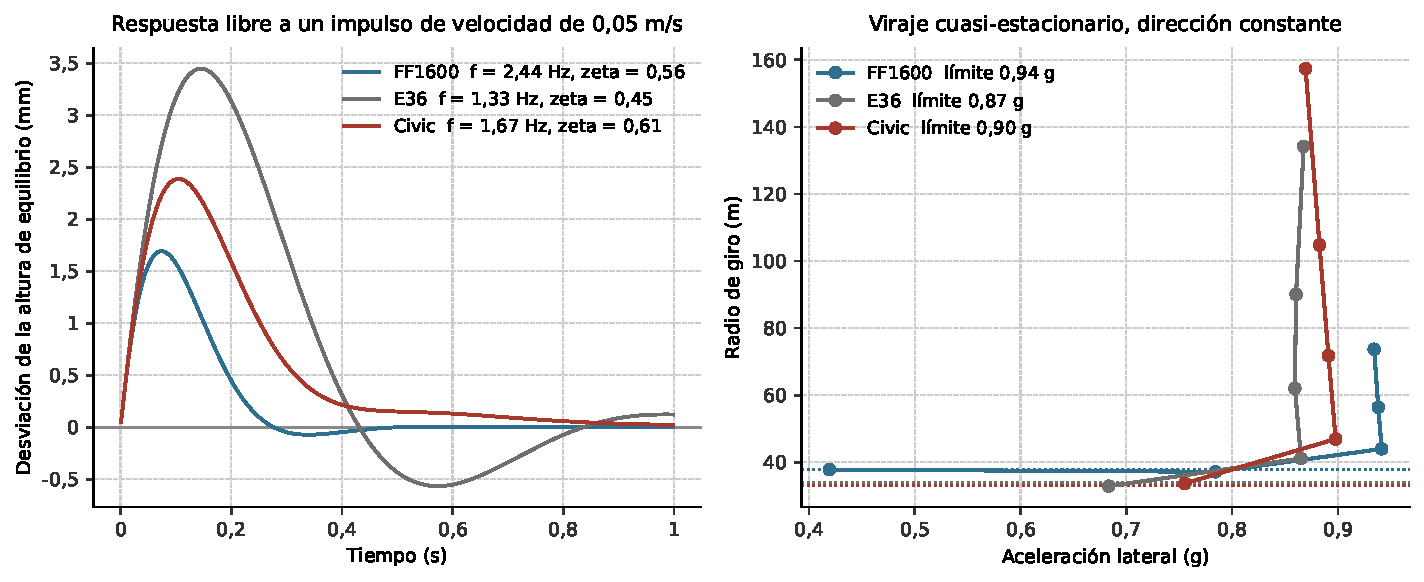
\includegraphics[width=\textwidth]{img/fidelidad.pdf}
\caption[Ensayos de fidelidad vertical y lateral]{Izquierda: respuesta libre del modo vertical tras perturbar en $5$ mm el estado asentado, con la frecuencia natural y el amortiguamiento identificados. Derecha: radio de giro en función de la aceleración lateral con dirección constante, un punto por valor de acelerador. Las líneas punteadas marcan el radio de Ackermann de cada vehículo, referencia de viraje neutro.}
\label{fig:fidelidad}
\end{figure}

La característica obtenida es la correcta, a baja aceleración lateral el radio se mantiene casi constante y a partir de cierto punto crece abruptamente sin que la aceleración lateral aumente, esto se debe a que el vehículo comienza a subvirar porque el neumático alcanzó su límite de adherencia.

% La característica obtenida es la correcta en su forma. A baja aceleración lateral el radio se mantiene aproximadamente constante y algo por encima del radio de Ackermann, y a partir de cierto punto crece abruptamente sin que la aceleración lateral siga aumentando: el neumático ha alcanzado su límite de adherencia y el vehículo se abre, esto es, subvira en el límite. Es el comportamiento que corresponde y el deseable desde el punto de vista de la seguridad.

El límite lateral alcanzado es de  $0{,}85$ g para el FF1600, $0{,}77$ g para el E36 y $0{,}85$ g para el Civic. Cabe aclarar que es un límite combinado y no puramente lateral, ya que al aplicar acelerador parte del presupuesto de agarre va también a la aceleración. Para un vehículo de calle sobre asfalto seco estos valores son válidos, sin embargo, para el monoplaza resultan bajos \cite{hyperphysics_tires}. Esto se debe a que el modelo de neumático utilizado fue el mismo para los tres vehículos, si se quisiera obtener un valor más preciso, habría que obtener y aplicar los parámetros de un neumático de competición.

% El ángulo de balanceo resulta remarcable. Los dos vehículos de calle se inclinan alrededor de $9$ grados por cada g de aceleración lateral (el E36 $6{,}8$ grados a $0{,}76$ g y el Civic $7{,}7$ a $0{,}82$ g) aproximadamente el doble de los $4$ a $5$ de un automóvil real. El monoplaza, con $3{,}3$ grados por g, queda donde corresponde.

% La causa es que no se implementó un modelo de barra estabilizadora, elemento del que un automóvil de calles obtiene buena parte de su resistencia al balanceo, lo que le permite montar resortes más blandos sin inclinarse demasiado al girar. El monoplaza no presenta esta falla debido a que un vehículo de competición si obtiene esa rigidez de resortes duros.  Agregarla es la corrección de fidelidad lateral más directa después de solucionar el reparto de pesos.


% El límite lateral alcanzado es de $0{,}74$ g para el FF1600, $0{,}70$ g para el E36 y $0{,}87$ g para el Civic. Conviene precisar que se trata de un límite combinado y no puramente lateral, puesto que el acelerador está aplicado y consume parte del presupuesto del círculo de fricción. Para un vehículo de calle sobre asfalto seco estos valores son verosímiles; para el monoplaza, en cambio, resultan bajos, ya que un vehículo de competición con neumáticos de compuesto blando supera holgadamente $1$ g.

% No fue posible extraer el gradiente de subviraje en el rango lineal. La resolución de acelerador disponible sitúa al vehículo por encima de $0{,}25$ g ya con el segundo valor ensayado, de modo que no se reúnen suficientes puntos por debajo del límite para ajustar una recta con sentido. Obtenerlo requeriría un regulador de velocidad que permitiera fijar pares (velocidad, radio) arbitrarios, lo que queda como trabajo pendiente.

\subsection{Distancia de frenado}

La prueba para verificar el comportamiento longitudinal consiste en acelerar y frenar a fondo luego de un tiempo determinado. Dado que este modelo no modela el downforce, la resistencia aerodinámica es menor, y tampoco tiene en cuenta la deformación del neumático, la frenada debe tener una desaceleración cercana al $1$ g, debido a que la carga normal del vehículo es solo su peso.

\begin{table}[H]
\centering
\begin{tabular}{lccccc}
\hline
Modelo & $v_0$ (km/h) & Distancia (m) & $a$ media (m/s$^2$) & $a$ media (g) & $a$ pico (m/s$^2$) \\
\hline
FF1600 & $93$  & $32{,}5$ & $10{,}18$ & $1{,}04$ & $10{,}92$ \\
E36    & $116$ & $51{,}4$ & $10{,}06$ & $1{,}03$ & $10{,}54$ \\
Civic  & $119$ & $54{,}6$ & $10{,}09$ & $1{,}03$ & $10{,}65$ \\
\hline
\end{tabular}
\caption[Distancia de frenado]{Frenada a fondo desde la velocidad indicada hasta la detención. La desaceleración media se calcula como $v_0^2 / 2d$.}
\label{tab:frenada}
\end{table}

Los resultados son consistentes con la cota mencionada anteriormente. Las desaceleraciones  medias del E36, Civic y FF1600 se sitúan justo sobre el límite de adherencia, superando el $1$ g debido al pico del inicio de la frenada. Las distancias resultantes coinciden con lo esperable.

% El monoplaza se detiene con una aceleración media menor, a pesa de que tiene el mismo coeficiente de fricción. Esto se debe a que la frenada no llega a alcanzar el agarre máximo de los neumáticos con el par que se le aplica, probablemente debido al menor peso del chasis. Si se quiere alcanzar una mejor frenada, se puede simplemente aumentar el parámetro de par máximo en el modelo para poder alcanzar el límite de adherencia.

Los valores pico superan la cota mencionada anteriormente porque corresponden a momentos transitorios en el momento de aplicar el freno, cuando la transferencia de pesos por el cabeceo del chasis incrementa la carga normal en el eje delantero, además de que la resistencia aerodinámica y de rodadura están más presentas a altas velocidades.



\subsection{Síntesis}

Tres de los cuatro ensayos dan resultados satisfactorios y el cuarto identifica una limitación concreta.

La contabilidad de las masas cierra con un error menor al $1{,}5\%$ con respecto a la suma de las masas declaradas, lo que valida la ley de contacto, la propagación del radio del neumático y el ensamblaje completo del vehículo. El comportamiento en frenada se corresponde a la cota del coeficiente de fricción y tiene valores coherentes con vehículos reales. El ensayo vertical sitúa tanto al E36 como al FF1600 dentro del rango esperado para la clase de vehículos que son.

La principal limitación es el reparto de cargas entre ejes, que es uniforme cuando no necesariamente debería serlo, esto es una consecuencia directa de modelar el chasis como un paralelepípedo con distribución de masa uniforme. Esta simplificación es la que más afecta al balance del vehículo y limita la fidelidad del comportamiento lateral. Una modificación en esta representación mejoraría la fidelidad significativamente.

% A esta limitación también se suma la ausencia de barras estabilizadoras: los dos vehículos de calle presentan un balanceo equivalente aproximadamente al doble del de un vehículo real. Agregar este componente es la segunda corrección en orden de importancia para mejorar la fidelidad, particularmente del viraje lateral.

% A ella se suma, en el mismo plano lateral, la ausencia de barra estabilizadora: con la vía en su valor correcto, los dos vehículos de calle acusan un gradiente de balanceo cercano a los $9$ grados por g, aproximadamente el doble del de un automóvil real, y en el límite su suspensión exterior alcanza los topes de compresión. Es la segunda corrección en orden de importancia, y no añade estados al sistema, ya que una barra estabilizadora es un resorte torsional entre las dos ruedas de un eje.

% A esto se suma una

% La limitación es el reparto de cargas entre ejes, uniforme cuando debería no serlo, consecuencia directa de modelar el chasis como un cuerpo de masa homogénea. Dado que ese reparto gobierna el balance del vehículo, es la simplificación que más acota la fidelidad lateral del modelo. A ella se suma, en el mismo plano lateral, una vía del orden de un $40\,\%$ mayor que la real en los tres vehículos, que sobreestima la rigidez al balanceo y obliga a leer los límites laterales medidos como optimistas. Son las dos magnitudes cuyo ajuste rendiría la mayor mejora de fidelidad, y ninguna de las dos exige cambios estructurales: la primera pide un chasis con centro de masa desplazado, la segunda un juego de anclajes y longitudes de brazo tomados del vehículo real.

Además quedan dos observaciones menos importantes: El Civic presenta una relación de instalación de $1{,}24$ cuando un automóvil real tiene alrededor de $0{,}5$ a $0{,}7$, lo que explica que la frecuencia vertical quede algo por fuera del rango de su tipo de vehículo. Revisar los puntos de anclaje del conjunto resorte-amortiguador, utilizando valores correspondientes a los reales debería corregir el problema sin modificar las rigideces declaradas. La otra observación es que en los tres modelos el amortiguamiento relativo excede el rango habitual.

Ninguna de estas limitaciones afecta a las conclusiones sobre desempeño de las secciones anteriores, pero si reducen la efectividad de su uso como simulador realista de conducción.

% Ninguna de estas limitaciones afecta a las conclusiones sobre desempeño de las secciones anteriores, que se refieren al costo y la exactitud de la integración y no al realismo del vehículo. Sí acotan, en cambio, el uso del simulador como herramienta de evaluación de comportamiento dinámico, y señalan con precisión qué habría que corregir para levantar esa restricción.

% Otra limitación, respecto al modelo de neumático, es que la fuerza lateral se modela como viscosa, proporcional a la velocidad lateral de deslizamiento, esto no tiene en cuenta, entre otras cosas la deformación del parche de contacto del neumático, ni el contacto de este en más de un punto del suelo. Esto se hizo para simplificar el sistema, debido a la complejidad que requiere desarrollar un modelo de neumáticos realista.

% Cabe añadir una limitación de fondo que estos ensayos ponen de manifiesto indirectamente. La fuerza lateral del neumático se modela como viscosa, proporcional a la velocidad lateral de deslizamiento, mientras que la de un neumático real es proporcional al ángulo de deriva, esto es, al cociente entre esa velocidad y la velocidad de avance. La consecuencia es que la rigidez de deriva efectiva del modelo crece de forma lineal con la velocidad en lugar de permanecer aproximadamente constante, lo que altera el balance del vehículo con la velocidad de un modo que no tiene contrapartida física. Sustituir la ley viscosa por un modelo basado en ángulo de deriva es, de todas las mejoras identificadas, la que más incidiría en la fidelidad del comportamiento lateral.
